% This is samplepaper.tex, a sample paper demonstrating the
% LLNCS class package for the SMU Data Science Review Journal;
%
% This sample paper is a modified version of samplepaper.tex for
% the Springer Computer Science proceedings; Version 2.20 of 2017/10/04
%
% Version 1.0 2019/06/03

% Use the llncs.cls formatting
\documentclass{llncs}

% Set the packages for use within the document. The following 
% packages should be included.  Additional packages that do not
% conflict with these packages or change the llncs class formatting
% may be used.  Packages that do change the formatting are
% not allowed.
\usepackage{graphicx} % Used for displaying a sample figure. 
% If possible, figure files should be included in EPS format. 
% PDF format is also acceptable. JPEG  will work, but some of 
% them are downsampled resulting in fuzzy images.
\usepackage{booktabs} % Better horizontal rules in tables
\usepackage{multirow} % Better combined rows in tables

% The title of the paper
\title{Increase Retention through Employee Advancement using Artificial Intelligence}

% The complete list of authors with their affiliations
\author{
Andy Ho\inst{1} \and
An Nguyen\inst{1} \and
Jodi Pafford\inst{1} \and
Dr. Robert Slater\inst{1}\and
Ame Ponce\inst{2}
}

% The Institutes and emails associated with each author. All students
% should use their MSDS affiliation or a generic SMU affiliation.
% Advisors should use their appropriate affiliation. Note that advisors
% are NOT referenced or otherwise denoted as advisors. Advisors
% are simply co-authors on the paper.
% Note that the emails for the MSDS affiliation, show how 
% to list emails that have the same organization portion.
\institute{
Master of Science in Data Science, Southern Methodist University,
Dallas TX 75275 USA 
\email{\{atho,angyuen2, jpafford, rslater\}@smu.edu} \and
Ernst \& Young, San Fransisco, California
\email{XXXXX@XXXXX.com} \\
% \url{http://www.springer.com/gp/computer-science/lncs}
}
% Begin the document
\begin{document}

\maketitle              % typeset the title and author of the paper

% Reset the footnote counter
\setcounter{footnote}{0}
% The abstract environment uses the \begin{} and \end{} constructs to 
% denote the beginning and ending of the abstract contents.
\begin{abstract}
The broad objective of this research is to increase retention through employee advancement using Artificial Intelligence by predicting the fit of an employee to an open role. The most valuable assets for businesses and organizations are its knowledgeable and trained employees. An estimated seventy-seven percent of attrition can be preventable by employers with one of the main reasons why employees move on is to pursue another opportunity for growth and a chance for higher pay. Losing employees is costly and finding a replacement externally is time consuming with no certainties of success. In analyzing job descriptions and employee evaluations with various algorithms in Natural Language Processing (NLP), Machine Learning (ML), and Deep Learning (DL), a predictive match index will be generated to score internal candidates for positions without employees needing to actively apply. The position could then be offered or recommended to employees. The hypothesis is by providing internal opportunities to qualified employees, the rate of retention will increase - leading to many positive outcomes for businesses and organizations such as increased profitability, improved culture and higher employee satisfaction.

% Keywords may be used, but they are not required.
%\keywords{First keyword  \and Second keyword \and Another keyword.}
\end{abstract}

% Sections are denoted by the use of the \section{Section Name} 
% command -- where "Section Name" is the name you give to the Section.
\section{Introduction}

Employees are vital resources for all companies and organizations.  It is a strategic issue and competitive advantage for businesses to retain quality or high performing employees as long as possible.  The time and cost associated to hiring new personnel includes recruiting, interviewing, training, and activities to cultivate a positive environment – keeping employees motivated.

The skill and knowledge of an employee is the key human capital for businesses to operate successfully and optimally.  When an employee leaves a company, a knowledge and experience gap is created, requiring companies to post job openings to the public to fill those gaps.  The average duration to find a replacement is 42 days.  In most cases, it takes five interviews to make an offer to an individual – often times needing to repeat the interview process multiple times to fully bring on board a new employee.

Over the past decades, more companies in general are experiencing a higher rate of attrition.  Individuals are looking for more opportunities for growth or higher salary, doing so sooner.  In 2018, the median employee tenure was 4.2 years.  The maximum median was of those between ages of 55 to 64 at 10.1 years and the minimum median of those between the ages of 25 to 34 at 2.8 years. ~\cite{article1} This disparity between the older and younger generation of workers is more than three times.  As the older generation retires, it is of increasing importance to address the low retention rate for the younger generation of workers.

In this research, Artificial Intelligence (AI) will be used to present a viable solution to increase employee retention of a company by matching existing employees to open roles.  There are many proposed definitions of AI but most share the same thread of understanding – the concept of computer programs capable of intelligence exhibited by humans. ~\cite{book1} This is a very generic definition to a complex technology.  The paper will provide a high-level but focus on the algorithms and techniques used within AI to demonstrate our methodology of solving the problem of attrition.

Natural Language Processing (NLP) is a branch of AI that helps machines understand, interpret, analyze, and manipulate human language.  NLP will be used on open role descriptions, employee evaluations, and any unstructured data.  In those cases, NLP will generate structured data to be used in Machine Learning and Deep Learning.

Machine Learning (ML) is another branch of AI that utilizes algorithms and statistical models to perform specific tasks.  ML has two main task types (Supervised and Unsupervised) with algorithms created for four specific purposes:
    \begin{enumerate}
      \item Regressions: Linear Regression, Ordinary Least Squares Regression, Local Regression, Neural Networks
      \item Classification: Decision Trees, K-Nearest Neighbor, Support Vector Machine, Logistice Regression, Naïve Bayes, Random Forests
      \item Cluster Analysis: K-Mean Clustering, Hierarchical Clustering
      \item Dimension Reduction: Principal Component Analysis, Linear Discriminant Analysis
    \end{enumerate}

Deep Learning (DL) is a subset of ML that teaches machines how to learn by mapping inputs to outputs to find correlations. Learning can be both supervised or unsupervised leveraging methods based on neural networks. DL is a key technology behind automated/autonomous devices such as driverless cars.

This paper is organized in the following: I. Introduction, II. Artificial Intelligence which will provide explanations of the algorithms and techniques, III. Methodology which is our recommended solution for the problem, IV. Related Work which is other published papers on attrition, V. Ethics and Feasibility addressing obstacles to solution deployment, VI. Conclusion and Future Work.

% Your first section should be your {\em Introduction} section. The Introduction is a 3--4 page executive summary of your paper.

% Note that paragraphs are created by placing a blank line before the 
% paragraph within the .tex file just as a blank line exists before the
% beginning of this comment. That blank line tells LaTeX to treat the 
% following text as a new paragraph.  No other commands are needed.
% The Introduction follows the same general organization as the Abstract.  

% The Introduction should have approximately 8--10 paragraphs.  The first paragraph is ``Motivation'' that states the broad problem and provides details as to why the problem is important. The second paragraph begins with the one sentence problem statement and then has 3--4 sentences adding details as needed.  There should then be 3--4 paragraphs detailing the final approach used to solve the problem.  Then a one paragraph summary of the main results followed by a one paragraph summary of the main conclusions.  The last paragraph should contain an overview of the remainder of the paper organization. 

% The Introduction section should {\bf NOT} contain tables, figures, or subsections.  This is a simple executive summary.

% A second section is begun with another \section{} command
\section{Artificial Intelligence}

% Subsections may be created with a \subsection{} command
\subsection{Subsection One}

Explanations of the algorithms and techniques will be found in this section.

\section{Methodology}

\subsection{Subsection One}

Recommended solution(s) for the problem.

\section{Related Work}

\subsection{Subsection One}

Other published papers on attrition.

Some published papers to add to the paper at a later time. \cite{article2,article3,article4}

\section{Ethics and Feasibility}

\subsection{Subsection One}

Addressing obstacles to solution deployment.

\section{Conclusion and Future Work}

\subsection{Subsection One}

Next steps based on findings.

% Please note that the first paragraph of a section or subsection is not indented. The first paragraph that follows a table, figure, equation etc. does not need an indent, either.

% Subsequent paragraphs, however, are indented.

% \subsubsection{Sample Heading (Third Level)} Only two levels of headings should be numbered. Lower level headings remain unnumbered; they are formatted as run-in headings.

% \paragraph{Sample Heading (Fourth Level)} The contribution should contain no more than four levels of headings. 

% Table~\ref{tab1} gives a summary of all heading levels. There should be zero reason to have either a 3rd-level heading or a 4th-level heading. If you feel the need to have such headings, then you should restructure your document such that no 3rd-level or 4th-level headings are needed.

% \begin{table}
% \caption{Table captions should be placed above the tables.}\label{tab1}
% \begin{tabular}{|l|l|l|}
% \hline
% Heading level &  Example & Font size and style\\
% \hline
% Title (centered) &  {\Large\bfseries Lecture Notes} & 14 point, bold\\
% 1st-level heading &  {\large\bfseries 1 Introduction} & 12 point, bold\\
% 2nd-level heading & {\bfseries 2.1 Printing Area} & 10 point, bold\\
% 3rd-level heading & {\bfseries Run-in Heading in Bold.} Text follows & 10 point, bold\\
% 4th-level heading & {\itshape Lowest Level Heading.} Text follows & 10 point, italic\\
% \hline
% \end{tabular}
% \end{table}


% While you should not need it, if a time comes when you need
% to force the beginning of a paragraph to not be indented, you 
% may use the \noindent command.

% Displayed and numbered equations such as Equation~\ref{eq:simpleEquation} are centered and set on a separate line.
% \begin{equation}
% \label{eq:simpleEquation}
% x + y = z
% \end{equation}

% Please try to avoid rasterized images for line-art diagrams and schemas. Whenever possible, use vector graphics instead (see
% Fig.~\ref{fig1}).

% \begin{figure}
% 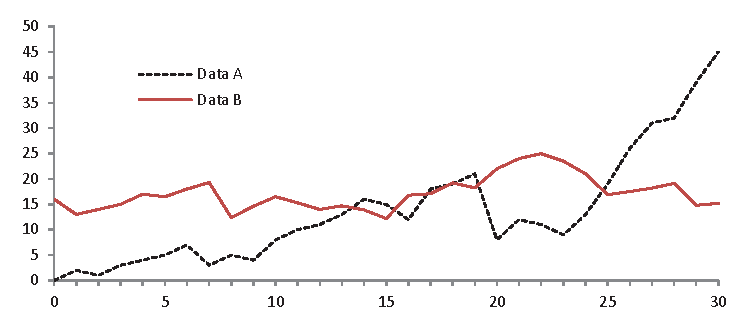
\includegraphics[width=\textwidth]{fig1.eps}
% \caption{A figure caption is always placed below the illustration.
% Please note that short captions are centered, while long ones are justified by the macro package automatically.} \label{fig1}
% \end{figure}

% \begin{theorem}
% This is a sample theorem. The run-in heading is set in bold, while the following text appears in italics. Definitions, lemmas, propositions, and corollaries are styled the same way.
% \end{theorem}
%
% the environments 'definition', 'lemma', 'proposition', 'corollary',
% 'remark', and 'example' are defined in the LLNCS documentclass as well.
%
% \begin{proof}
% Proofs, examples, and remarks have the initial word in italics, while the following text appears in normal font.
% \end{proof}

% For citations of references, we prefer the use of square brackets and consecutive numbers where the references are numbered according to the ascending alphabet (i.e.,~a to z) of the first author's last name. Citations using labels or the author/year convention are not acceptable. The following reference provides a sample reference list with entries for journal articles~\cite{article1,article2}, a chapter~ cite{inbook}, a book~\cite{book}, and a conference proceedings without editors~\cite{conference}.
%%% Multiple citations are grouped \cite{article1,article2,inbook,book,conference}.

% Note that URLs should be placed in Footnotes\footnote{More information may be found at \url{http://www.smu.edu}. Last accessed 31 Dec 2018.} and not in the references.  Only documents that will not change over time should be placed in the references and cited.
%
% ---- Bibliography ----
%
% BibTeX users should specify bibliography style 'splncs04'.
% References will then be sorted according to alphabetical 
% and formatted in the correct style.
%
 \bibliographystyle{splncs04}
 \bibliography{samplebib}

% End the document
\end{document}
